\section{Speech Tokens and Language Model Pipelines}

\begin{frame}{Neural Audio Codecs: Audio as Tokens}
  \begin{itemize}
    \item Neural audio codecs compress a waveform into a short sequence of \textbf{discrete tokens} and reconstruct audio from them: SoundStream (Zeghidour et al., 2021) and EnCodec (D\'efossez et al., 2022).
    \item An encoder downsamples the waveform, \textbf{residual vector quantization} maps each frame to entries of learned codebooks, and a decoder reconstructs the waveform from the codes.
    \item The result: audio becomes a token sequence, the same kind of object a language model already consumes and produces.
  \end{itemize}
  \begin{figure}
    \centering
    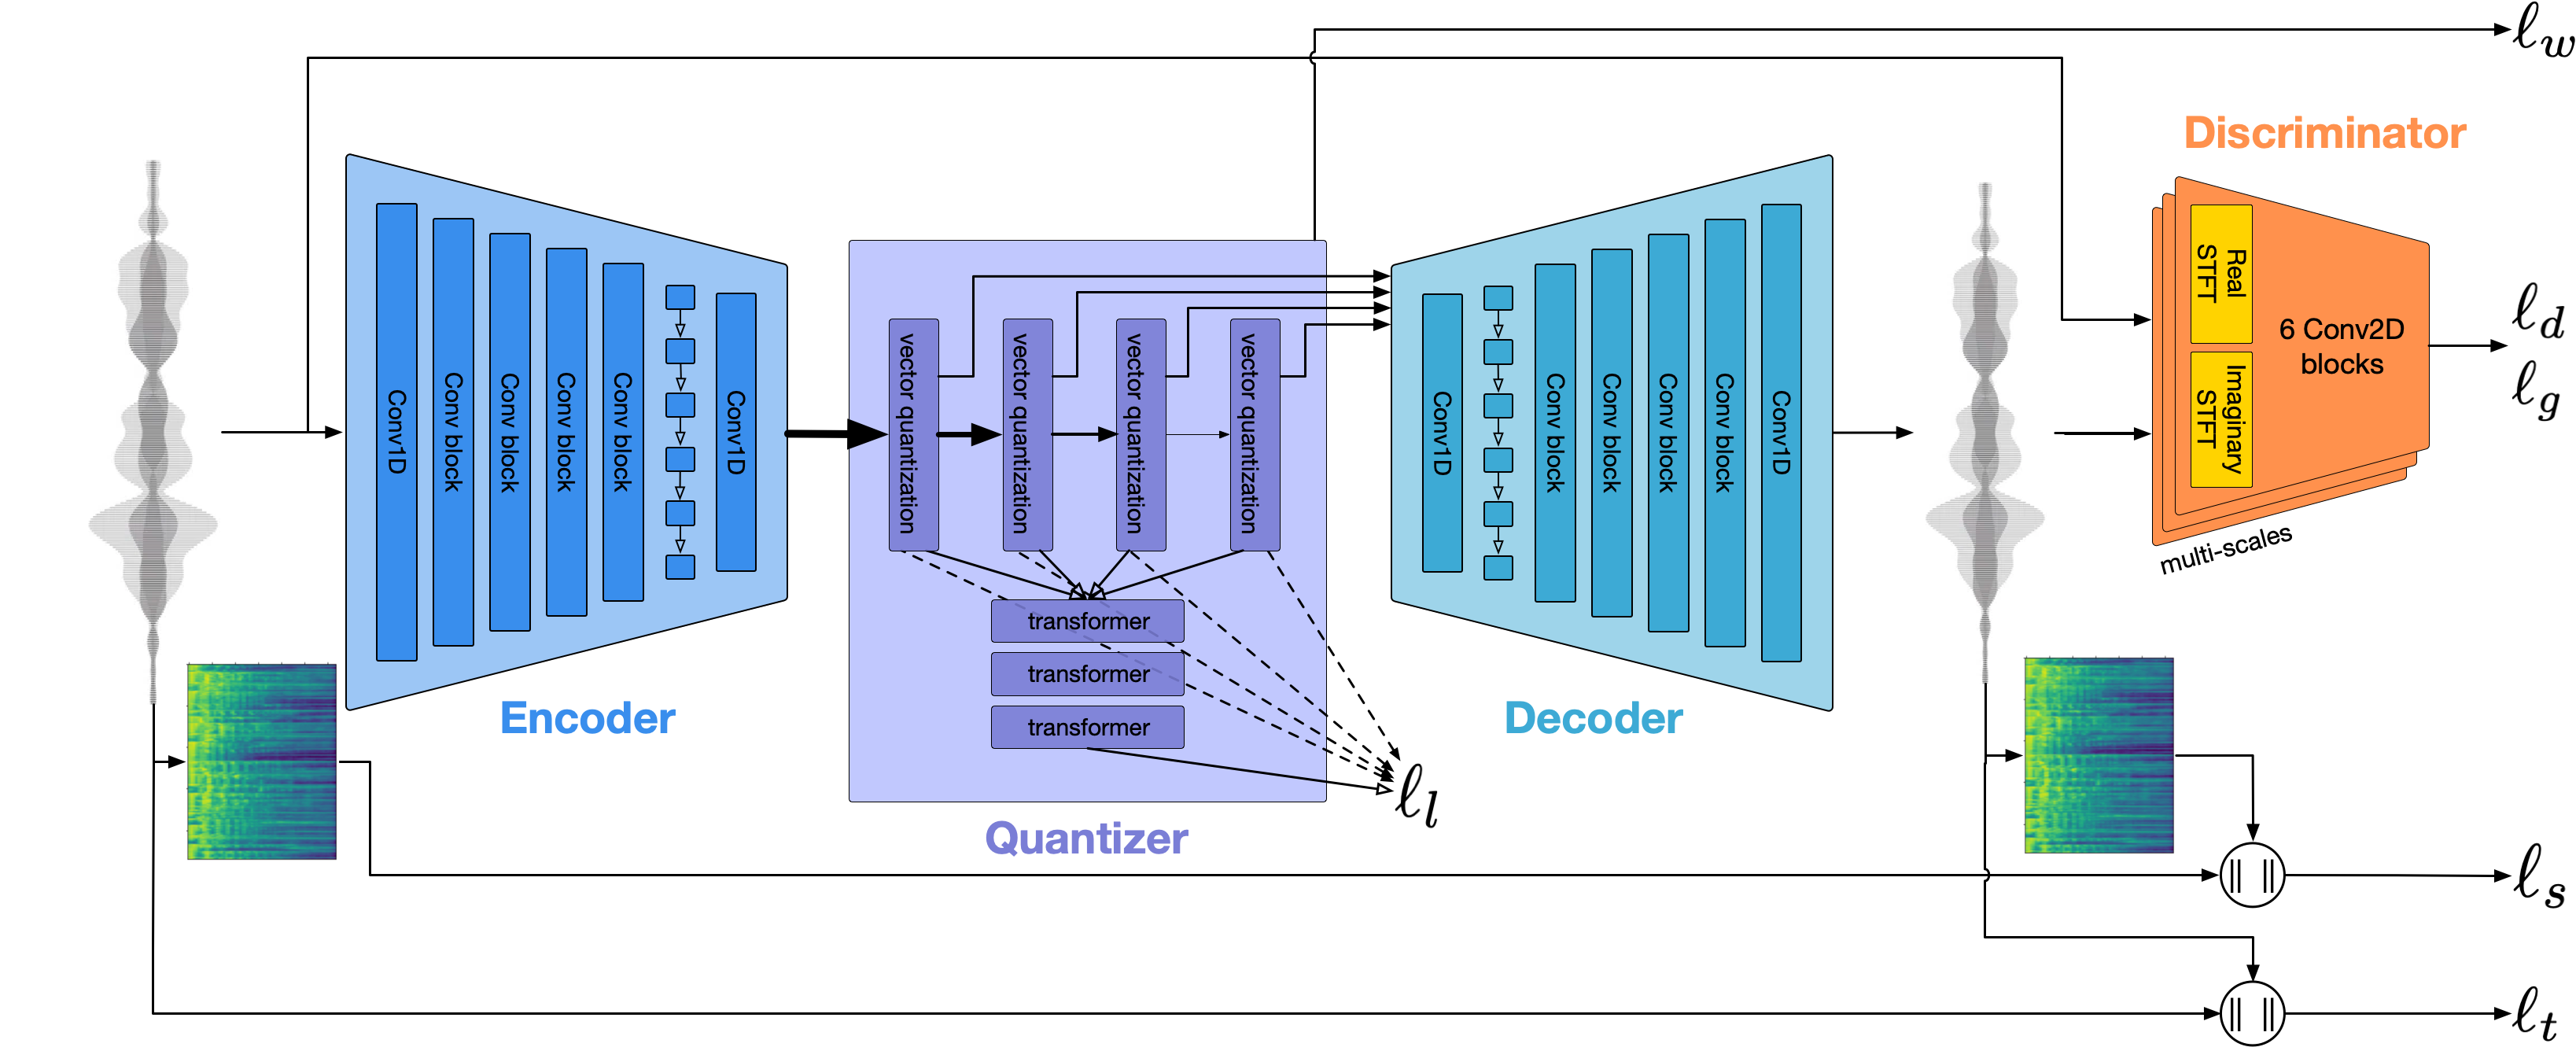
\includegraphics[width=0.85\textwidth,height=0.5\textheight,keepaspectratio]{images/tts/encodec_architecture_rvq_codec.png}
    \caption*{EnCodec: encoder, residual vector quantizer, and decoder. Source: \href{https://github.com/facebookresearch/encodec}{D\'efossez et al. (2022)}}
  \end{figure}
\end{frame}

\begin{frame}{Speech in the Language Model Pipeline}
  \begin{itemize}
    \item Once audio is tokens, speech tasks become language modeling. VALL-E is the TTS instance: predict codec tokens conditioned on text and a short voice prompt.
    \item \textbf{AudioLM} (Borsos et al., 2022) showed pure audio continuation: a decoder-only model over audio tokens that continues speech or music with no text at all.
    \item \textbf{Speech-LLMs} put both directions in one model: ASR is audio tokens in, text out; TTS is text in, audio tokens out; the same transformer serves both.
    \item End-to-end voice conversation models take this to its conclusion: speech tokens in, speech tokens out, with no intermediate text transcript required.
  \end{itemize}
\end{frame}

\begin{frame}{Why Token Pipelines Beat Cascades}
  \begin{itemize}
    \item The classic voice assistant is a \textbf{cascade}: ASR $\rightarrow$ text LLM $\rightarrow$ TTS, three models and two conversions per turn.
    \item \textbf{Latency:} each stage waits for the previous one; a single token-level model can start responding while still listening.
    \item \textbf{Information loss:} a transcript discards tone, emphasis, emotion, and speaker identity; token pipelines keep them end to end.
    \item \textbf{Error compounding:} an ASR mistake becomes unrecoverable once only text is passed on.
    \item Cascades still win on modularity and controllability, which is why both designs coexist in production.
  \end{itemize}
\end{frame}
